\documentclass[1p]{elsarticle_modified}
%\bibliographystyle{elsarticle-num}

%\usepackage[colorlinks]{hyperref}
%\usepackage{abbrmath_seonhwa} %\Abb, \Ascr, \Acal ,\Abf, \Afrak
\usepackage{amsfonts}
\usepackage{amssymb}
\usepackage{amsmath}
\usepackage{amsthm}
\usepackage{scalefnt}
\usepackage{amsbsy}
\usepackage{kotex}
\usepackage{caption}
\usepackage{subfig}
\usepackage{color}
\usepackage{graphicx}
\usepackage{xcolor} %% white, black, red, green, blue, cyan, magenta, yellow
\usepackage{float}
\usepackage{setspace}
\usepackage{hyperref}

\usepackage{tikz}
\usetikzlibrary{arrows}

\usepackage{multirow}
\usepackage{array} % fixed length table
\usepackage{hhline}

%%%%%%%%%%%%%%%%%%%%%
\makeatletter
\renewcommand*\env@matrix[1][\arraystretch]{%
	\edef\arraystretch{#1}%
	\hskip -\arraycolsep
	\let\@ifnextchar\new@ifnextchar
	\array{*\c@MaxMatrixCols c}}
\makeatother %https://tex.stackexchange.com/questions/14071/how-can-i-increase-the-line-spacing-in-a-matrix
%%%%%%%%%%%%%%%

\usepackage[normalem]{ulem}

\newcommand{\msout}[1]{\ifmmode\text{\sout{\ensuremath{#1}}}\else\sout{#1}\fi}
%SOURCE: \msout is \stkout macro in https://tex.stackexchange.com/questions/20609/strikeout-in-math-mode

\newcommand{\cancel}[1]{
	\ifmmode
	{\color{red}\msout{#1}}
	\else
	{\color{red}\sout{#1}}
	\fi
}

\newcommand{\add}[1]{
	{\color{blue}\uwave{#1}}
}

\newcommand{\replace}[2]{
	\ifmmode
	{\color{red}\msout{#1}}{\color{blue}\uwave{#2}}
	\else
	{\color{red}\sout{#1}}{\color{blue}\uwave{#2}}
	\fi
}

\newcommand{\Sol}{\mathcal{S}} %segment
\newcommand{\D}{D} %diagram
\newcommand{\A}{\mathcal{A}} %arc


%%%%%%%%%%%%%%%%%%%%%%%%%%%%%5 test

\def\sl{\operatorname{\textup{SL}}(2,\Cbb)}
\def\psl{\operatorname{\textup{PSL}}(2,\Cbb)}
\def\quan{\mkern 1mu \triangleright \mkern 1mu}

\theoremstyle{definition}
\newtheorem{thm}{Theorem}[section]
\newtheorem{prop}[thm]{Proposition}
\newtheorem{lem}[thm]{Lemma}
\newtheorem{ques}[thm]{Question}
\newtheorem{cor}[thm]{Corollary}
\newtheorem{defn}[thm]{Definition}
\newtheorem{exam}[thm]{Example}
\newtheorem{rmk}[thm]{Remark}
\newtheorem{alg}[thm]{Algorithm}

\newcommand{\I}{\sqrt{-1}}
\begin{document}

%\begin{frontmatter}
%
%\title{Boundary parabolic representations of knots up to 8 crossings}
%
%%% Group authors per affiliation:
%\author{Yunhi Cho} 
%\address{Department of Mathematics, University of Seoul, Seoul, Korea}
%\ead{yhcho@uos.ac.kr}
%
%
%\author{Seonhwa Kim} %\fnref{s_kim}}
%\address{Center for Geometry and Physics, Institute for Basic Science, Pohang, 37673, Korea}
%\ead{ryeona17@ibs.re.kr}
%
%\author{Hyuk Kim}
%\address{Department of Mathematical Sciences, Seoul National University, Seoul 08826, Korea}
%\ead{hyukkim@snu.ac.kr}
%
%\author{Seokbeom Yoon}
%\address{Department of Mathematical Sciences, Seoul National University, Seoul, 08826,  Korea}
%\ead{sbyoon15@snu.ac.kr}
%
%\begin{abstract}
%We find all boundary parabolic representation of knots up to 8 crossings.
%
%\end{abstract}
%\begin{keyword}
%    \MSC[2010] 57M25 
%\end{keyword}
%
%\end{frontmatter}

%\linenumbers
%\tableofcontents
%
\newcommand\colored[1]{\textcolor{white}{\rule[-0.35ex]{0.8em}{1.4ex}}\kern-0.8em\color{red} #1}%
%\newcommand\colored[1]{\textcolor{white}{ #1}\kern-2.17ex	\textcolor{white}{ #1}\kern-1.81ex	\textcolor{white}{ #1}\kern-2.15ex\color{red}#1	}

{\Large $\underline{12n_{0076}~(K12n_{0076})}$}

\setlength{\tabcolsep}{10pt}
\renewcommand{\arraystretch}{1.6}
\vspace{1cm}\begin{tabular}{m{100pt}>{\centering\arraybackslash}m{274pt}}
\multirow{5}{120pt}{
	\centering
	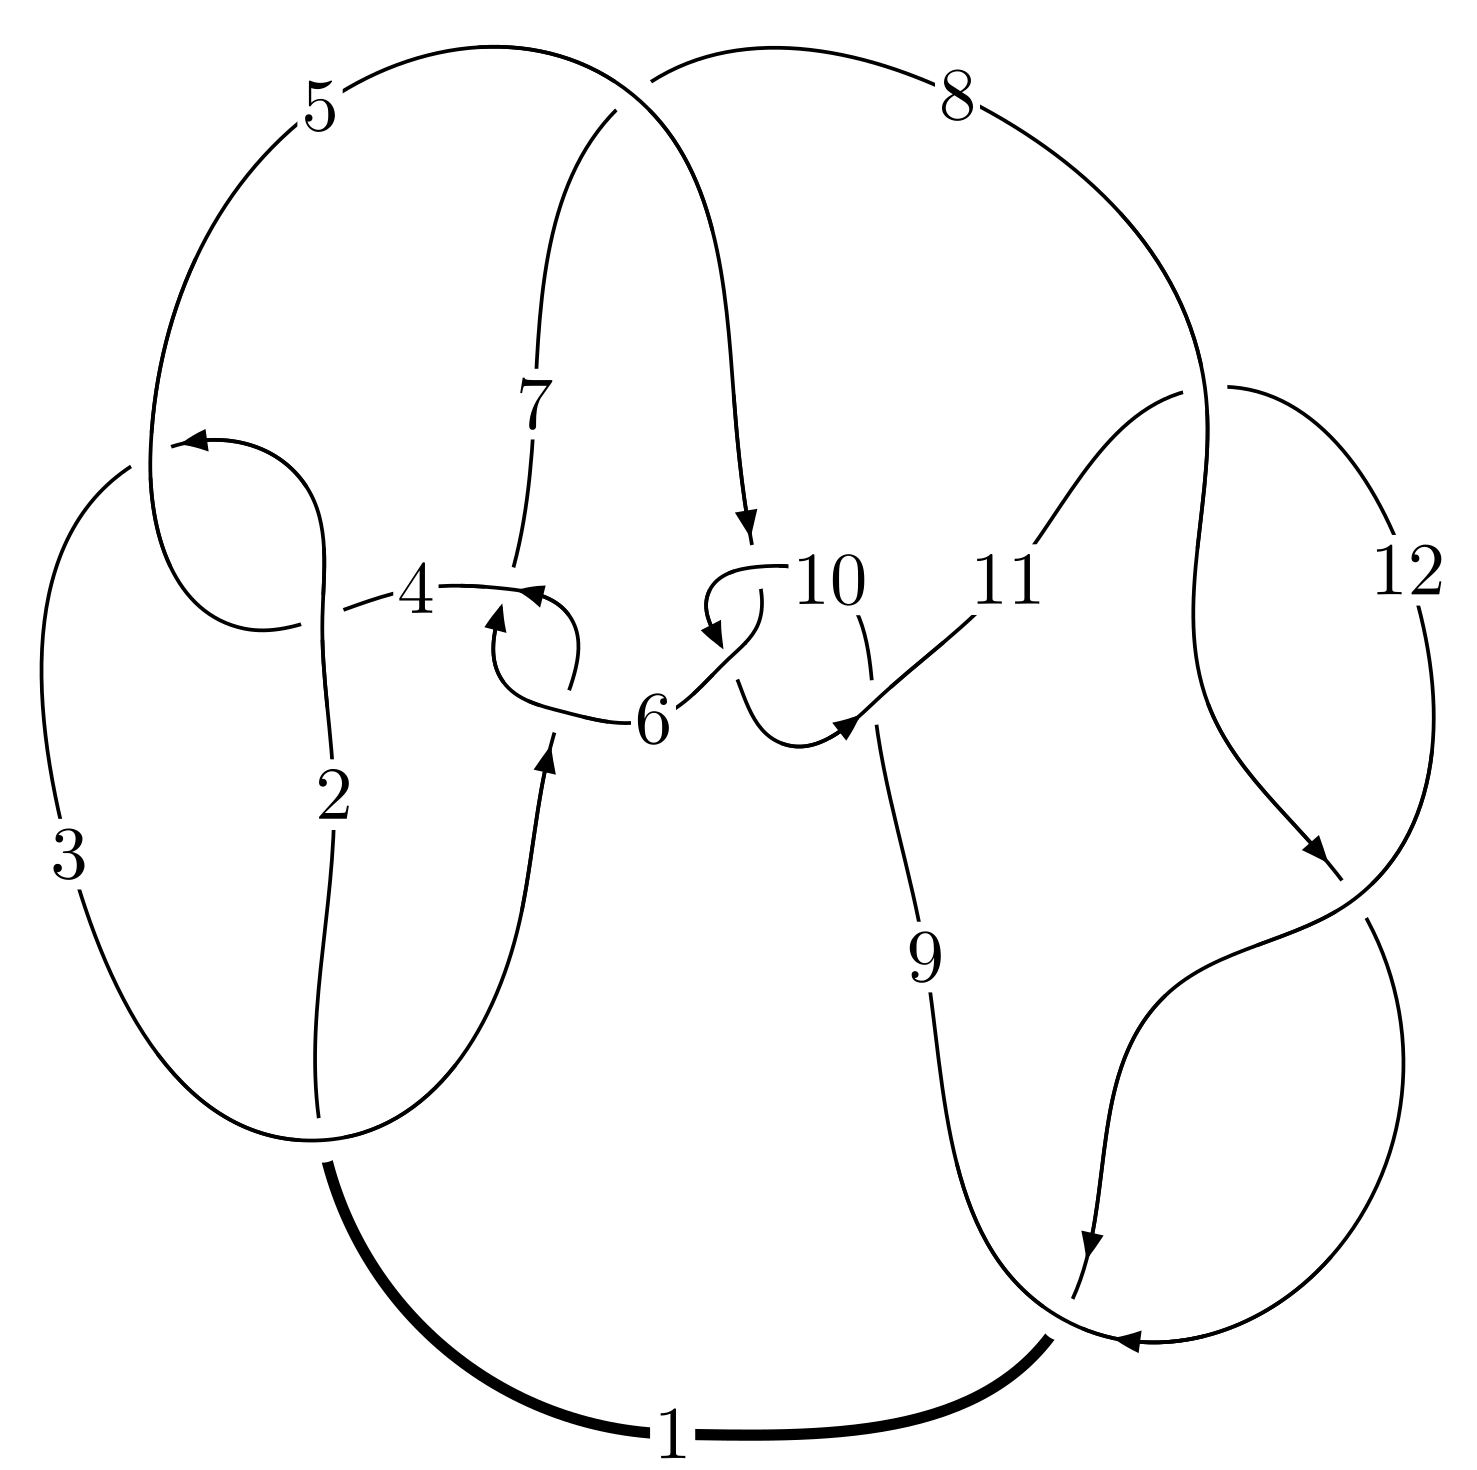
\includegraphics[width=112pt]{../../../GIT/diagram.site/Diagrams/png/2165_12n_0076.png}\\
\ \ \ A knot diagram\footnotemark}&
\allowdisplaybreaks
\textbf{Linearized knot diagam} \\
\cline{2-2}
 &
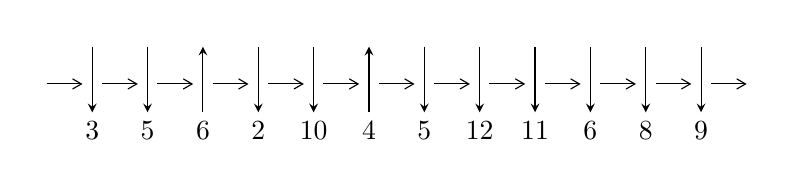
\begin{tikzpicture}[x=20pt, y=17pt]
	% nodes
	\node (C0) at (0, 0) {};
	\node (C1) at (1, 0) {};
	\node (C1U) at (1, +1) {};
	\node (C1D) at (1, -1) {3};

	\node (C2) at (2, 0) {};
	\node (C2U) at (2, +1) {};
	\node (C2D) at (2, -1) {5};

	\node (C3) at (3, 0) {};
	\node (C3U) at (3, +1) {};
	\node (C3D) at (3, -1) {6};

	\node (C4) at (4, 0) {};
	\node (C4U) at (4, +1) {};
	\node (C4D) at (4, -1) {2};

	\node (C5) at (5, 0) {};
	\node (C5U) at (5, +1) {};
	\node (C5D) at (5, -1) {10};

	\node (C6) at (6, 0) {};
	\node (C6U) at (6, +1) {};
	\node (C6D) at (6, -1) {4};

	\node (C7) at (7, 0) {};
	\node (C7U) at (7, +1) {};
	\node (C7D) at (7, -1) {5};

	\node (C8) at (8, 0) {};
	\node (C8U) at (8, +1) {};
	\node (C8D) at (8, -1) {12};

	\node (C9) at (9, 0) {};
	\node (C9U) at (9, +1) {};
	\node (C9D) at (9, -1) {11};

	\node (C10) at (10, 0) {};
	\node (C10U) at (10, +1) {};
	\node (C10D) at (10, -1) {6};

	\node (C11) at (11, 0) {};
	\node (C11U) at (11, +1) {};
	\node (C11D) at (11, -1) {8};

	\node (C12) at (12, 0) {};
	\node (C12U) at (12, +1) {};
	\node (C12D) at (12, -1) {9};
	\node (C13) at (13, 0) {};

	% arrows
	\draw[->,>={angle 60}]
	(C0) edge (C1) (C1) edge (C2) (C2) edge (C3) (C3) edge (C4) (C4) edge (C5) (C5) edge (C6) (C6) edge (C7) (C7) edge (C8) (C8) edge (C9) (C9) edge (C10) (C10) edge (C11) (C11) edge (C12) (C12) edge (C13) ;	\draw[->,>=stealth]
	(C1U) edge (C1D) (C2U) edge (C2D) (C3D) edge (C3U) (C4U) edge (C4D) (C5U) edge (C5D) (C6D) edge (C6U) (C7U) edge (C7D) (C8U) edge (C8D) (C9U) edge (C9D) (C10U) edge (C10D) (C11U) edge (C11D) (C12U) edge (C12D) ;
	\end{tikzpicture} \\
\hhline{~~} \\& 
\textbf{Solving Sequence} \\ \cline{2-2} 
 &
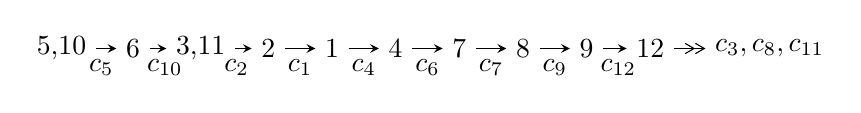
\begin{tikzpicture}[x=23pt, y=7pt]
	% node
	\node (A0) at (-1/8, 0) {5,10};
	\node (A1) at (1, 0) {6};
	\node (A2) at (33/16, 0) {3,11};
	\node (A3) at (25/8, 0) {2};
	\node (A4) at (33/8, 0) {1};
	\node (A5) at (41/8, 0) {4};
	\node (A6) at (49/8, 0) {7};
	\node (A7) at (57/8, 0) {8};
	\node (A8) at (65/8, 0) {9};
	\node (A9) at (73/8, 0) {12};
	\node (C1) at (1/2, -1) {$c_{5}$};
	\node (C2) at (3/2, -1) {$c_{10}$};
	\node (C3) at (21/8, -1) {$c_{2}$};
	\node (C4) at (29/8, -1) {$c_{1}$};
	\node (C5) at (37/8, -1) {$c_{4}$};
	\node (C6) at (45/8, -1) {$c_{6}$};
	\node (C7) at (53/8, -1) {$c_{7}$};
	\node (C8) at (61/8, -1) {$c_{9}$};
	\node (C9) at (69/8, -1) {$c_{12}$};
	\node (A10) at (11, 0) {$c_{3},c_{8},c_{11}$};

	% edge
	\draw[->,>=stealth]	
	(A0) edge (A1) (A1) edge (A2) (A2) edge (A3) (A3) edge (A4) (A4) edge (A5) (A5) edge (A6) (A6) edge (A7) (A7) edge (A8) (A8) edge (A9) ;
	\draw[->>,>={angle 60}]	
	(A9) edge (A10);
\end{tikzpicture} \\ 

\end{tabular} \\

\footnotetext{
The image of knot diagram is generated by the software ``\textbf{Draw programme}" developed by Andrew Bartholomew(\url{http://www.layer8.co.uk/maths/draw/index.htm\#Running-draw}), where we modified some parts for our purpose(\url{https://github.com/CATsTAILs/LinksPainter}).
}\phantom \\ \newline 
\centering \textbf{Ideals for irreducible components\footnotemark of $X_{\text{par}}$} 
 
\begin{align*}
I^u_{1}&=\langle 
-1.99559\times10^{15} u^{33}+5.12786\times10^{15} u^{32}+\cdots+3.29400\times10^{15} b+2.31961\times10^{14},\\
\phantom{I^u_{1}}&\phantom{= \langle  }-6.21494\times10^{15} u^{33}+1.10612\times10^{16} u^{32}+\cdots+3.29400\times10^{15} a+8.86419\times10^{15},\;u^{34}-2 u^{33}+\cdots- u+1\rangle \\
I^u_{2}&=\langle 
b+1,\;2 u^7- u^6-3 u^5+3 u^4+4 u^3-3 u^2+a-2 u+4,\;u^8- u^7- u^6+2 u^5+u^4-2 u^3+2 u-1\rangle \\
\\
\end{align*}
\raggedright * 2 irreducible components of $\dim_{\mathbb{C}}=0$, with total 42 representations.\\
\footnotetext{All coefficients of polynomials are rational numbers. But the coefficients are sometimes approximated in decimal forms when there is not enough margin.}
\newpage
\renewcommand{\arraystretch}{1}
\centering \section*{I. $I^u_{1}= \langle -2.00\times10^{15} u^{33}+5.13\times10^{15} u^{32}+\cdots+3.29\times10^{15} b+2.32\times10^{14},\;-6.21\times10^{15} u^{33}+1.11\times10^{16} u^{32}+\cdots+3.29\times10^{15} a+8.86\times10^{15},\;u^{34}-2 u^{33}+\cdots- u+1 \rangle$}
\flushleft \textbf{(i) Arc colorings}\\
\begin{tabular}{m{7pt} m{180pt} m{7pt} m{180pt} }
\flushright $a_{5}=$&$\begin{pmatrix}1\\0\end{pmatrix}$ \\
\flushright $a_{10}=$&$\begin{pmatrix}0\\u\end{pmatrix}$ \\
\flushright $a_{6}=$&$\begin{pmatrix}1\\u^2\end{pmatrix}$ \\
\flushright $a_{3}=$&$\begin{pmatrix}1.88675 u^{33}-3.35800 u^{32}+\cdots-0.414433 u-2.69102\\0.605825 u^{33}-1.55673 u^{32}+\cdots-2.42216 u-0.0704193\end{pmatrix}$ \\
\flushright $a_{11}=$&$\begin{pmatrix}- u\\- u^3+u\end{pmatrix}$ \\
\flushright $a_{2}=$&$\begin{pmatrix}2.49257 u^{33}-4.91473 u^{32}+\cdots-2.83659 u-2.76144\\0.605825 u^{33}-1.55673 u^{32}+\cdots-2.42216 u-0.0704193\end{pmatrix}$ \\
\flushright $a_{1}=$&$\begin{pmatrix}0.684721 u^{33}-1.85986 u^{32}+\cdots-3.17571 u+0.213786\\-0.0613225 u^{33}+0.190476 u^{32}+\cdots+0.906554 u-0.351909\end{pmatrix}$ \\
\flushright $a_{4}=$&$\begin{pmatrix}2.09274 u^{33}-3.89228 u^{32}+\cdots-1.36534 u-2.34594\\0.572218 u^{33}-1.57386 u^{32}+\cdots-2.75044 u+0.0518727\end{pmatrix}$ \\
\flushright $a_{7}=$&$\begin{pmatrix}0.684721 u^{33}-1.85986 u^{32}+\cdots-3.17571 u+0.213786\\0.395472 u^{33}-0.984131 u^{32}+\cdots-2.08170 u+0.842330\end{pmatrix}$ \\
\flushright $a_{8}=$&$\begin{pmatrix}0.289249 u^{33}-0.875732 u^{32}+\cdots-1.09401 u-0.628544\\0.395472 u^{33}-0.984131 u^{32}+\cdots-2.08170 u+0.842330\end{pmatrix}$ \\
\flushright $a_{9}=$&$\begin{pmatrix}u^3\\u^5- u^3+u\end{pmatrix}$ \\
\flushright $a_{12}=$&$\begin{pmatrix}0.466506 u^{33}-1.30241 u^{32}+\cdots-2.66126 u+0.0407295\\-0.269323 u^{33}+0.553369 u^{32}+\cdots+1.71300 u-0.617147\end{pmatrix}$\\&\end{tabular}
\flushleft \textbf{(ii) Obstruction class $= -1$}\\~\\
\flushleft \textbf{(iii) Cusp Shapes $= -\frac{7661808169491132}{3293995579890413} u^{33}+\frac{6218879522456028}{3293995579890413} u^{32}+\cdots+\frac{25977556548692283}{3293995579890413} u-\frac{23126112688430199}{3293995579890413}$}\\~\\
\newpage\renewcommand{\arraystretch}{1}
\flushleft \textbf{(iv) u-Polynomials at the component}\newline \\
\begin{tabular}{m{50pt}|m{274pt}}
Crossings & \hspace{64pt}u-Polynomials at each crossing \\
\hline $$\begin{aligned}c_{1}\end{aligned}$$&$\begin{aligned}
&u^{34}+3 u^{33}+\cdots+71 u+1
\end{aligned}$\\
\hline $$\begin{aligned}c_{2},c_{4}\end{aligned}$$&$\begin{aligned}
&u^{34}-9 u^{33}+\cdots-15 u+1
\end{aligned}$\\
\hline $$\begin{aligned}c_{3},c_{6}\end{aligned}$$&$\begin{aligned}
&u^{34}+3 u^{33}+\cdots+2176 u+256
\end{aligned}$\\
\hline $$\begin{aligned}c_{5},c_{10}\end{aligned}$$&$\begin{aligned}
&u^{34}-2 u^{33}+\cdots- u+1
\end{aligned}$\\
\hline $$\begin{aligned}c_{7}\end{aligned}$$&$\begin{aligned}
&u^{34}-6 u^{33}+\cdots+1795665 u+338425
\end{aligned}$\\
\hline $$\begin{aligned}c_{8},c_{11},c_{12}\end{aligned}$$&$\begin{aligned}
&u^{34}-2 u^{33}+\cdots+7 u+1
\end{aligned}$\\
\hline $$\begin{aligned}c_{9}\end{aligned}$$&$\begin{aligned}
&u^{34}+6 u^{33}+\cdots+11 u+1
\end{aligned}$\\
\hline
\end{tabular}\\~\\
\newpage\renewcommand{\arraystretch}{1}
\flushleft \textbf{(v) Riley Polynomials at the component}\newline \\
\begin{tabular}{m{50pt}|m{274pt}}
Crossings & \hspace{64pt}Riley Polynomials at each crossing \\
\hline $$\begin{aligned}c_{1}\end{aligned}$$&$\begin{aligned}
&y^{34}+65 y^{33}+\cdots-5331 y+1
\end{aligned}$\\
\hline $$\begin{aligned}c_{2},c_{4}\end{aligned}$$&$\begin{aligned}
&y^{34}-3 y^{33}+\cdots-71 y+1
\end{aligned}$\\
\hline $$\begin{aligned}c_{3},c_{6}\end{aligned}$$&$\begin{aligned}
&y^{34}-51 y^{33}+\cdots-1228800 y+65536
\end{aligned}$\\
\hline $$\begin{aligned}c_{5},c_{10}\end{aligned}$$&$\begin{aligned}
&y^{34}-6 y^{33}+\cdots-11 y+1
\end{aligned}$\\
\hline $$\begin{aligned}c_{7}\end{aligned}$$&$\begin{aligned}
&y^{34}+106 y^{33}+\cdots+912331286925 y+114531480625
\end{aligned}$\\
\hline $$\begin{aligned}c_{8},c_{11},c_{12}\end{aligned}$$&$\begin{aligned}
&y^{34}-26 y^{33}+\cdots-11 y+1
\end{aligned}$\\
\hline $$\begin{aligned}c_{9}\end{aligned}$$&$\begin{aligned}
&y^{34}+46 y^{33}+\cdots+y+1
\end{aligned}$\\
\hline
\end{tabular}\\~\\
\newpage\flushleft \textbf{(vi) Complex Volumes and Cusp Shapes}
$$\begin{array}{c|c|c}  
\text{Solutions to }I^u_{1}& \I (\text{vol} + \sqrt{-1}CS) & \text{Cusp shape}\\
 \hline 
\begin{aligned}
u &= \phantom{-}0.635489 + 0.765565 I \\
a &= \phantom{-}0.023523 + 0.819812 I \\
b &= \phantom{-}0.143823 - 0.811670 I\end{aligned}
 & \phantom{-}3.05379 - 1.22135 I & -2.44643 + 1.78317 I \\ \hline\begin{aligned}
u &= \phantom{-}0.635489 - 0.765565 I \\
a &= \phantom{-}0.023523 - 0.819812 I \\
b &= \phantom{-}0.143823 + 0.811670 I\end{aligned}
 & \phantom{-}3.05379 + 1.22135 I & -2.44643 - 1.78317 I \\ \hline\begin{aligned}
u &= -0.729595 + 0.661430 I \\
a &= \phantom{-}0.034703 - 1.094050 I \\
b &= -0.136834 + 1.060550 I\end{aligned}
 & -0.23851 + 4.87038 I & -8.16084 - 6.79059 I \\ \hline\begin{aligned}
u &= -0.729595 - 0.661430 I \\
a &= \phantom{-}0.034703 + 1.094050 I \\
b &= -0.136834 - 1.060550 I\end{aligned}
 & -0.23851 - 4.87038 I & -8.16084 + 6.79059 I \\ \hline\begin{aligned}
u &= -0.479562 + 0.911974 I \\
a &= \phantom{-}0.046982 - 0.468540 I \\
b &= \phantom{-}0.371651 + 0.493500 I\end{aligned}
 & -1.11923 - 1.98539 I & -6.62012 + 2.37959 I \\ \hline\begin{aligned}
u &= -0.479562 - 0.911974 I \\
a &= \phantom{-}0.046982 + 0.468540 I \\
b &= \phantom{-}0.371651 - 0.493500 I\end{aligned}
 & -1.11923 + 1.98539 I & -6.62012 - 2.37959 I \\ \hline\begin{aligned}
u &= -0.766682 + 0.495753 I \\
a &= \phantom{-}1.50878 + 0.43111 I \\
b &= \phantom{-}0.146629 - 0.533111 I\end{aligned}
 & -0.524122 - 0.409066 I & -7.28048 - 0.84766 I \\ \hline\begin{aligned}
u &= -0.766682 - 0.495753 I \\
a &= \phantom{-}1.50878 - 0.43111 I \\
b &= \phantom{-}0.146629 + 0.533111 I\end{aligned}
 & -0.524122 + 0.409066 I & -7.28048 + 0.84766 I \\ \hline\begin{aligned}
u &= \phantom{-}0.971312 + 0.567163 I \\
a &= \phantom{-}1.103300 - 0.703542 I \\
b &= \phantom{-}0.496724 + 0.591318 I\end{aligned}
 & \phantom{-}1.85693 - 3.80699 I & -4.56903 + 5.73620 I \\ \hline\begin{aligned}
u &= \phantom{-}0.971312 - 0.567163 I \\
a &= \phantom{-}1.103300 + 0.703542 I \\
b &= \phantom{-}0.496724 - 0.591318 I\end{aligned}
 & \phantom{-}1.85693 + 3.80699 I & -4.56903 - 5.73620 I\\
 \hline 
 \end{array}$$\newpage$$\begin{array}{c|c|c}  
\text{Solutions to }I^u_{1}& \I (\text{vol} + \sqrt{-1}CS) & \text{Cusp shape}\\
 \hline 
\begin{aligned}
u &= \phantom{-}1.17100\phantom{ +0.000000I} \\
a &= \phantom{-}0.851526\phantom{ +0.000000I} \\
b &= \phantom{-}0.548404\phantom{ +0.000000I}\end{aligned}
 & -7.23479\phantom{ +0.000000I} & -9.88000\phantom{ +0.000000I} \\ \hline\begin{aligned}
u &= \phantom{-}0.718624 + 0.314023 I \\
a &= \phantom{-}0.116591 + 1.245780 I \\
b &= -1.100530 - 0.643963 I\end{aligned}
 & -4.65847 - 3.05078 I & -14.9930 + 6.5224 I \\ \hline\begin{aligned}
u &= \phantom{-}0.718624 - 0.314023 I \\
a &= \phantom{-}0.116591 - 1.245780 I \\
b &= -1.100530 + 0.643963 I\end{aligned}
 & -4.65847 + 3.05078 I & -14.9930 - 6.5224 I \\ \hline\begin{aligned}
u &= -1.123410 + 0.599536 I \\
a &= \phantom{-}0.797874 + 0.695393 I \\
b &= \phantom{-}0.704883 - 0.508995 I\end{aligned}
 & -3.27432 + 7.58793 I & -9.23689 - 7.74257 I \\ \hline\begin{aligned}
u &= -1.123410 - 0.599536 I \\
a &= \phantom{-}0.797874 - 0.695393 I \\
b &= \phantom{-}0.704883 + 0.508995 I\end{aligned}
 & -3.27432 - 7.58793 I & -9.23689 + 7.74257 I \\ \hline\begin{aligned}
u &= -0.721712\phantom{ +0.000000I} \\
a &= -0.340670\phantom{ +0.000000I} \\
b &= -1.45745\phantom{ +0.000000I}\end{aligned}
 & -6.03886\phantom{ +0.000000I} & -17.6920\phantom{ +0.000000I} \\ \hline\begin{aligned}
u &= \phantom{-}0.900311 + 0.952119 I \\
a &= -0.732531 + 0.736305 I \\
b &= \phantom{-}0.96904 - 1.25880 I\end{aligned}
 & \phantom{-}9.10120 - 4.37771 I & -7.49633 + 3.28771 I \\ \hline\begin{aligned}
u &= \phantom{-}0.900311 - 0.952119 I \\
a &= -0.732531 - 0.736305 I \\
b &= \phantom{-}0.96904 + 1.25880 I\end{aligned}
 & \phantom{-}9.10120 + 4.37771 I & -7.49633 - 3.28771 I \\ \hline\begin{aligned}
u &= -0.905172 + 0.980418 I \\
a &= -0.763195 - 0.646287 I \\
b &= \phantom{-}1.05364 + 1.18320 I\end{aligned}
 & \phantom{-}12.90170 - 0.67521 I & -4.51148 - 0.04928 I \\ \hline\begin{aligned}
u &= -0.905172 - 0.980418 I \\
a &= -0.763195 + 0.646287 I \\
b &= \phantom{-}1.05364 - 1.18320 I\end{aligned}
 & \phantom{-}12.90170 + 0.67521 I & -4.51148 + 0.04928 I\\
 \hline 
 \end{array}$$\newpage$$\begin{array}{c|c|c}  
\text{Solutions to }I^u_{1}& \I (\text{vol} + \sqrt{-1}CS) & \text{Cusp shape}\\
 \hline 
\begin{aligned}
u &= \phantom{-}0.995190 + 0.896687 I \\
a &= \phantom{-}0.62305 - 1.64005 I \\
b &= \phantom{-}1.05804 + 1.11835 I\end{aligned}
 & \phantom{-}8.78395 - 2.42502 I & -7.89113 + 1.48359 I \\ \hline\begin{aligned}
u &= \phantom{-}0.995190 - 0.896687 I \\
a &= \phantom{-}0.62305 + 1.64005 I \\
b &= \phantom{-}1.05804 - 1.11835 I\end{aligned}
 & \phantom{-}8.78395 + 2.42502 I & -7.89113 - 1.48359 I \\ \hline\begin{aligned}
u &= \phantom{-}0.901655 + 1.007390 I \\
a &= -0.755401 + 0.558173 I \\
b &= \phantom{-}1.09702 - 1.08890 I\end{aligned}
 & \phantom{-}8.64740 + 5.63592 I & -8.00000 - 2.80908 I \\ \hline\begin{aligned}
u &= \phantom{-}0.901655 - 1.007390 I \\
a &= -0.755401 - 0.558173 I \\
b &= \phantom{-}1.09702 + 1.08890 I\end{aligned}
 & \phantom{-}8.64740 - 5.63592 I & -8.00000 + 2.80908 I \\ \hline\begin{aligned}
u &= -0.530883 + 0.364299 I \\
a &= \phantom{-}0.43019 - 1.79437 I \\
b &= -0.779658 + 0.298976 I\end{aligned}
 & -1.01260 + 1.22984 I & -7.99935 - 4.73307 I \\ \hline\begin{aligned}
u &= -0.530883 - 0.364299 I \\
a &= \phantom{-}0.43019 + 1.79437 I \\
b &= -0.779658 - 0.298976 I\end{aligned}
 & -1.01260 - 1.22984 I & -7.99935 + 4.73307 I \\ \hline\begin{aligned}
u &= -1.012560 + 0.914952 I \\
a &= \phantom{-}0.49655 + 1.65048 I \\
b &= \phantom{-}1.15087 - 1.09510 I\end{aligned}
 & \phantom{-}12.5409 + 7.6268 I & -5.13159 - 4.40800 I \\ \hline\begin{aligned}
u &= -1.012560 - 0.914952 I \\
a &= \phantom{-}0.49655 - 1.65048 I \\
b &= \phantom{-}1.15087 + 1.09510 I\end{aligned}
 & \phantom{-}12.5409 - 7.6268 I & -5.13159 + 4.40800 I \\ \hline\begin{aligned}
u &= -0.620369\phantom{ +0.000000I} \\
a &= \phantom{-}1.18712\phantom{ +0.000000I} \\
b &= \phantom{-}0.117070\phantom{ +0.000000I}\end{aligned}
 & -0.969949\phantom{ +0.000000I} & -9.86690\phantom{ +0.000000I} \\ \hline\begin{aligned}
u &= \phantom{-}1.031790 + 0.924118 I \\
a &= \phantom{-}0.39495 - 1.60999 I \\
b &= \phantom{-}1.21367 + 1.04076 I\end{aligned}
 & \phantom{-}8.2072 - 12.7003 I & -8.60420 + 6.93082 I\\
 \hline 
 \end{array}$$\newpage$$\begin{array}{c|c|c}  
\text{Solutions to }I^u_{1}& \I (\text{vol} + \sqrt{-1}CS) & \text{Cusp shape}\\
 \hline 
\begin{aligned}
u &= \phantom{-}1.031790 - 0.924118 I \\
a &= \phantom{-}0.39495 + 1.60999 I \\
b &= \phantom{-}1.21367 - 1.04076 I\end{aligned}
 & \phantom{-}8.2072 + 12.7003 I & -8.60420 - 6.93082 I \\ \hline\begin{aligned}
u &= \phantom{-}0.246676 + 0.443752 I \\
a &= \phantom{-}4.30323 + 2.74241 I \\
b &= -0.948262 + 0.125356 I\end{aligned}
 & -3.28757 + 0.51694 I & -12.3807 + 13.4722 I \\ \hline\begin{aligned}
u &= \phantom{-}0.246676 - 0.443752 I \\
a &= \phantom{-}4.30323 - 2.74241 I \\
b &= -0.948262 - 0.125356 I\end{aligned}
 & -3.28757 - 0.51694 I & -12.3807 - 13.4722 I \\ \hline\begin{aligned}
u &= \phantom{-}0.464719\phantom{ +0.000000I} \\
a &= -2.95516\phantom{ +0.000000I} \\
b &= -1.08945\phantom{ +0.000000I}\end{aligned}
 & -2.17611\phantom{ +0.000000I} & \phantom{-}3.01310\phantom{ +0.000000I}\\
 \hline 
 \end{array}$$\newpage\newpage\renewcommand{\arraystretch}{1}
\centering \section*{II. $I^u_{2}= \langle b+1,\;2 u^7- u^6-3 u^5+3 u^4+4 u^3-3 u^2+a-2 u+4,\;u^8- u^7- u^6+2 u^5+u^4-2 u^3+2 u-1 \rangle$}
\flushleft \textbf{(i) Arc colorings}\\
\begin{tabular}{m{7pt} m{180pt} m{7pt} m{180pt} }
\flushright $a_{5}=$&$\begin{pmatrix}1\\0\end{pmatrix}$ \\
\flushright $a_{10}=$&$\begin{pmatrix}0\\u\end{pmatrix}$ \\
\flushright $a_{6}=$&$\begin{pmatrix}1\\u^2\end{pmatrix}$ \\
\flushright $a_{3}=$&$\begin{pmatrix}-2 u^7+u^6+3 u^5-3 u^4-4 u^3+3 u^2+2 u-4\\-1\end{pmatrix}$ \\
\flushright $a_{11}=$&$\begin{pmatrix}- u\\- u^3+u\end{pmatrix}$ \\
\flushright $a_{2}=$&$\begin{pmatrix}-2 u^7+u^6+3 u^5-3 u^4-4 u^3+3 u^2+2 u-5\\-1\end{pmatrix}$ \\
\flushright $a_{1}=$&$\begin{pmatrix}-1\\0\end{pmatrix}$ \\
\flushright $a_{4}=$&$\begin{pmatrix}-2 u^7+u^6+3 u^5-3 u^4-4 u^3+3 u^2+2 u-4\\-1\end{pmatrix}$ \\
\flushright $a_{7}=$&$\begin{pmatrix}1\\u^2\end{pmatrix}$ \\
\flushright $a_{8}=$&$\begin{pmatrix}- u^2+1\\u^2\end{pmatrix}$ \\
\flushright $a_{9}=$&$\begin{pmatrix}u^3\\u^5- u^3+u\end{pmatrix}$ \\
\flushright $a_{12}=$&$\begin{pmatrix}u^7-2 u^5+2 u^3-2 u\\- u^7+u^5-2 u^3+u\end{pmatrix}$\\&\end{tabular}
\flushleft \textbf{(ii) Obstruction class $= 1$}\\~\\
\flushleft \textbf{(iii) Cusp Shapes $= -10 u^7+2 u^6+16 u^5-12 u^4-19 u^3+9 u^2+8 u-27$}\\~\\
\newpage\renewcommand{\arraystretch}{1}
\flushleft \textbf{(iv) u-Polynomials at the component}\newline \\
\begin{tabular}{m{50pt}|m{274pt}}
Crossings & \hspace{64pt}u-Polynomials at each crossing \\
\hline $$\begin{aligned}c_{1},c_{2}\end{aligned}$$&$\begin{aligned}
&(u-1)^8
\end{aligned}$\\
\hline $$\begin{aligned}c_{3},c_{6}\end{aligned}$$&$\begin{aligned}
&u^8
\end{aligned}$\\
\hline $$\begin{aligned}c_{4}\end{aligned}$$&$\begin{aligned}
&(u+1)^8
\end{aligned}$\\
\hline $$\begin{aligned}c_{5}\end{aligned}$$&$\begin{aligned}
&u^8- u^7- u^6+2 u^5+u^4-2 u^3+2 u-1
\end{aligned}$\\
\hline $$\begin{aligned}c_{7}\end{aligned}$$&$\begin{aligned}
&u^8+3 u^7+7 u^6+10 u^5+11 u^4+10 u^3+6 u^2+4 u+1
\end{aligned}$\\
\hline $$\begin{aligned}c_{8}\end{aligned}$$&$\begin{aligned}
&u^8+u^7-3 u^6-2 u^5+3 u^4+2 u-1
\end{aligned}$\\
\hline $$\begin{aligned}c_{9}\end{aligned}$$&$\begin{aligned}
&u^8-3 u^7+7 u^6-10 u^5+11 u^4-10 u^3+6 u^2-4 u+1
\end{aligned}$\\
\hline $$\begin{aligned}c_{10}\end{aligned}$$&$\begin{aligned}
&u^8+u^7- u^6-2 u^5+u^4+2 u^3-2 u-1
\end{aligned}$\\
\hline $$\begin{aligned}c_{11},c_{12}\end{aligned}$$&$\begin{aligned}
&u^8- u^7-3 u^6+2 u^5+3 u^4-2 u-1
\end{aligned}$\\
\hline
\end{tabular}\\~\\
\newpage\renewcommand{\arraystretch}{1}
\flushleft \textbf{(v) Riley Polynomials at the component}\newline \\
\begin{tabular}{m{50pt}|m{274pt}}
Crossings & \hspace{64pt}Riley Polynomials at each crossing \\
\hline $$\begin{aligned}c_{1},c_{2},c_{4}\end{aligned}$$&$\begin{aligned}
&(y-1)^8
\end{aligned}$\\
\hline $$\begin{aligned}c_{3},c_{6}\end{aligned}$$&$\begin{aligned}
&y^8
\end{aligned}$\\
\hline $$\begin{aligned}c_{5},c_{10}\end{aligned}$$&$\begin{aligned}
&y^8-3 y^7+7 y^6-10 y^5+11 y^4-10 y^3+6 y^2-4 y+1
\end{aligned}$\\
\hline $$\begin{aligned}c_{7},c_{9}\end{aligned}$$&$\begin{aligned}
&y^8+5 y^7+11 y^6+6 y^5-17 y^4-34 y^3-22 y^2-4 y+1
\end{aligned}$\\
\hline $$\begin{aligned}c_{8},c_{11},c_{12}\end{aligned}$$&$\begin{aligned}
&y^8-7 y^7+19 y^6-22 y^5+3 y^4+14 y^3-6 y^2-4 y+1
\end{aligned}$\\
\hline
\end{tabular}\\~\\
\newpage\flushleft \textbf{(vi) Complex Volumes and Cusp Shapes}
$$\begin{array}{c|c|c}  
\text{Solutions to }I^u_{2}& \I (\text{vol} + \sqrt{-1}CS) & \text{Cusp shape}\\
 \hline 
\begin{aligned}
u &= \phantom{-}0.570868 + 0.730671 I \\
a &= \phantom{-}0.281371 + 1.128550 I \\
b &= -1.00000\phantom{ +0.000000I}\end{aligned}
 & -2.68559 + 1.13123 I & -9.56807 - 0.79885 I \\ \hline\begin{aligned}
u &= \phantom{-}0.570868 - 0.730671 I \\
a &= \phantom{-}0.281371 - 1.128550 I \\
b &= -1.00000\phantom{ +0.000000I}\end{aligned}
 & -2.68559 - 1.13123 I & -9.56807 + 0.79885 I \\ \hline\begin{aligned}
u &= -0.855237 + 0.665892 I \\
a &= -0.208670 - 0.825203 I \\
b &= -1.00000\phantom{ +0.000000I}\end{aligned}
 & \phantom{-}0.51448 + 2.57849 I & -6.42531 - 3.25625 I \\ \hline\begin{aligned}
u &= -0.855237 - 0.665892 I \\
a &= -0.208670 + 0.825203 I \\
b &= -1.00000\phantom{ +0.000000I}\end{aligned}
 & \phantom{-}0.51448 - 2.57849 I & -6.42531 + 3.25625 I \\ \hline\begin{aligned}
u &= -1.09818\phantom{ +0.000000I} \\
a &= -0.829189\phantom{ +0.000000I} \\
b &= -1.00000\phantom{ +0.000000I}\end{aligned}
 & -8.14766\phantom{ +0.000000I} & -20.0060\phantom{ +0.000000I} \\ \hline\begin{aligned}
u &= \phantom{-}1.031810 + 0.655470 I \\
a &= -0.284386 + 0.605794 I \\
b &= -1.00000\phantom{ +0.000000I}\end{aligned}
 & -4.02461 - 6.44354 I & -11.71592 + 3.92092 I \\ \hline\begin{aligned}
u &= \phantom{-}1.031810 - 0.655470 I \\
a &= -0.284386 - 0.605794 I \\
b &= -1.00000\phantom{ +0.000000I}\end{aligned}
 & -4.02461 + 6.44354 I & -11.71592 - 3.92092 I \\ \hline\begin{aligned}
u &= \phantom{-}0.603304\phantom{ +0.000000I} \\
a &= -2.74744\phantom{ +0.000000I} \\
b &= -1.00000\phantom{ +0.000000I}\end{aligned}
 & -2.48997\phantom{ +0.000000I} & -23.5750\phantom{ +0.000000I}\\
 \hline 
 \end{array}$$\newpage
\newpage\renewcommand{\arraystretch}{1}
\centering \section*{ III. u-Polynomials}
\begin{tabular}{m{50pt}|m{274pt}}
Crossings & \hspace{64pt}u-Polynomials at each crossing \\
\hline $$\begin{aligned}c_{1}\end{aligned}$$&$\begin{aligned}
&((u-1)^8)(u^{34}+3 u^{33}+\cdots+71 u+1)
\end{aligned}$\\
\hline $$\begin{aligned}c_{2}\end{aligned}$$&$\begin{aligned}
&((u-1)^8)(u^{34}-9 u^{33}+\cdots-15 u+1)
\end{aligned}$\\
\hline $$\begin{aligned}c_{3},c_{6}\end{aligned}$$&$\begin{aligned}
&u^8(u^{34}+3 u^{33}+\cdots+2176 u+256)
\end{aligned}$\\
\hline $$\begin{aligned}c_{4}\end{aligned}$$&$\begin{aligned}
&((u+1)^8)(u^{34}-9 u^{33}+\cdots-15 u+1)
\end{aligned}$\\
\hline $$\begin{aligned}c_{5}\end{aligned}$$&$\begin{aligned}
&(u^8- u^7+\cdots+2 u-1)(u^{34}-2 u^{33}+\cdots- u+1)
\end{aligned}$\\
\hline $$\begin{aligned}c_{7}\end{aligned}$$&$\begin{aligned}
&(u^8+3 u^7+7 u^6+10 u^5+11 u^4+10 u^3+6 u^2+4 u+1)\\
&\cdot(u^{34}-6 u^{33}+\cdots+1795665 u+338425)
\end{aligned}$\\
\hline $$\begin{aligned}c_{8}\end{aligned}$$&$\begin{aligned}
&(u^8+u^7-3 u^6-2 u^5+3 u^4+2 u-1)(u^{34}-2 u^{33}+\cdots+7 u+1)
\end{aligned}$\\
\hline $$\begin{aligned}c_{9}\end{aligned}$$&$\begin{aligned}
&(u^8-3 u^7+7 u^6-10 u^5+11 u^4-10 u^3+6 u^2-4 u+1)\\
&\cdot(u^{34}+6 u^{33}+\cdots+11 u+1)
\end{aligned}$\\
\hline $$\begin{aligned}c_{10}\end{aligned}$$&$\begin{aligned}
&(u^8+u^7+\cdots-2 u-1)(u^{34}-2 u^{33}+\cdots- u+1)
\end{aligned}$\\
\hline $$\begin{aligned}c_{11},c_{12}\end{aligned}$$&$\begin{aligned}
&(u^8- u^7-3 u^6+2 u^5+3 u^4-2 u-1)(u^{34}-2 u^{33}+\cdots+7 u+1)
\end{aligned}$\\
\hline
\end{tabular}\newpage\renewcommand{\arraystretch}{1}
\centering \section*{ IV. Riley Polynomials}
\begin{tabular}{m{50pt}|m{274pt}}
Crossings & \hspace{64pt}Riley Polynomials at each crossing \\
\hline $$\begin{aligned}c_{1}\end{aligned}$$&$\begin{aligned}
&((y-1)^8)(y^{34}+65 y^{33}+\cdots-5331 y+1)
\end{aligned}$\\
\hline $$\begin{aligned}c_{2},c_{4}\end{aligned}$$&$\begin{aligned}
&((y-1)^8)(y^{34}-3 y^{33}+\cdots-71 y+1)
\end{aligned}$\\
\hline $$\begin{aligned}c_{3},c_{6}\end{aligned}$$&$\begin{aligned}
&y^8(y^{34}-51 y^{33}+\cdots-1228800 y+65536)
\end{aligned}$\\
\hline $$\begin{aligned}c_{5},c_{10}\end{aligned}$$&$\begin{aligned}
&(y^8-3 y^7+7 y^6-10 y^5+11 y^4-10 y^3+6 y^2-4 y+1)\\
&\cdot(y^{34}-6 y^{33}+\cdots-11 y+1)
\end{aligned}$\\
\hline $$\begin{aligned}c_{7}\end{aligned}$$&$\begin{aligned}
&(y^8+5 y^7+11 y^6+6 y^5-17 y^4-34 y^3-22 y^2-4 y+1)\\
&\cdot(y^{34}+106 y^{33}+\cdots+912331286925 y+114531480625)
\end{aligned}$\\
\hline $$\begin{aligned}c_{8},c_{11},c_{12}\end{aligned}$$&$\begin{aligned}
&(y^8-7 y^7+19 y^6-22 y^5+3 y^4+14 y^3-6 y^2-4 y+1)\\
&\cdot(y^{34}-26 y^{33}+\cdots-11 y+1)
\end{aligned}$\\
\hline $$\begin{aligned}c_{9}\end{aligned}$$&$\begin{aligned}
&(y^8+5 y^7+11 y^6+6 y^5-17 y^4-34 y^3-22 y^2-4 y+1)\\
&\cdot(y^{34}+46 y^{33}+\cdots+y+1)
\end{aligned}$\\
\hline
\end{tabular}
\vskip 2pc
\end{document}